\chapter{PLANIFICATION DES TRAJECTOIRES}

\section{Path and trajectory planning}

\subsection{Définitions}

Le \textbf{path planning} (planification de chemin) consiste à déterminer un \textbf{chemin géométrique} reliant un point initial à un point final, en passant éventuellement par des points de passage intermédiaires (\textit{via-points}). Ce chemin est une courbe purement spatiale, définie dans l'espace articulaire ou dans l'espace opérationnel du robot. Il s'agit de savoir « par où passe le robot » sans aucune référence au temps, à la vitesse ou à l'accélération \cite{gasparetto2015}.

Le \textbf{trajectory planning} (planification de trajectoire) prend ce chemin géométrique comme donnée d'entrée et y \textbf{associe une information temporelle} : à quel instant le robot doit se trouver à chaque point du chemin, avec quelle vitesse et quelle accélération \cite{gasparetto2015}.

Elle conditionne directement la qualité du mouvement : le choix des temps de passage aux \textit{via-points} influence non seulement les propriétés \textbf{cinématiques} du mouvement (vitesse, accélération), mais aussi ses propriétés \textbf{dynamiques}, les efforts inertiels subis par le robot dépendent des accélérations, et les vibrations de sa structure mécanique sont déterminées par les valeurs du \textbf{jerk} (dérivée de l'accélération) \cite{gasparetto2015}.

\begin{figure}[H]
\centering
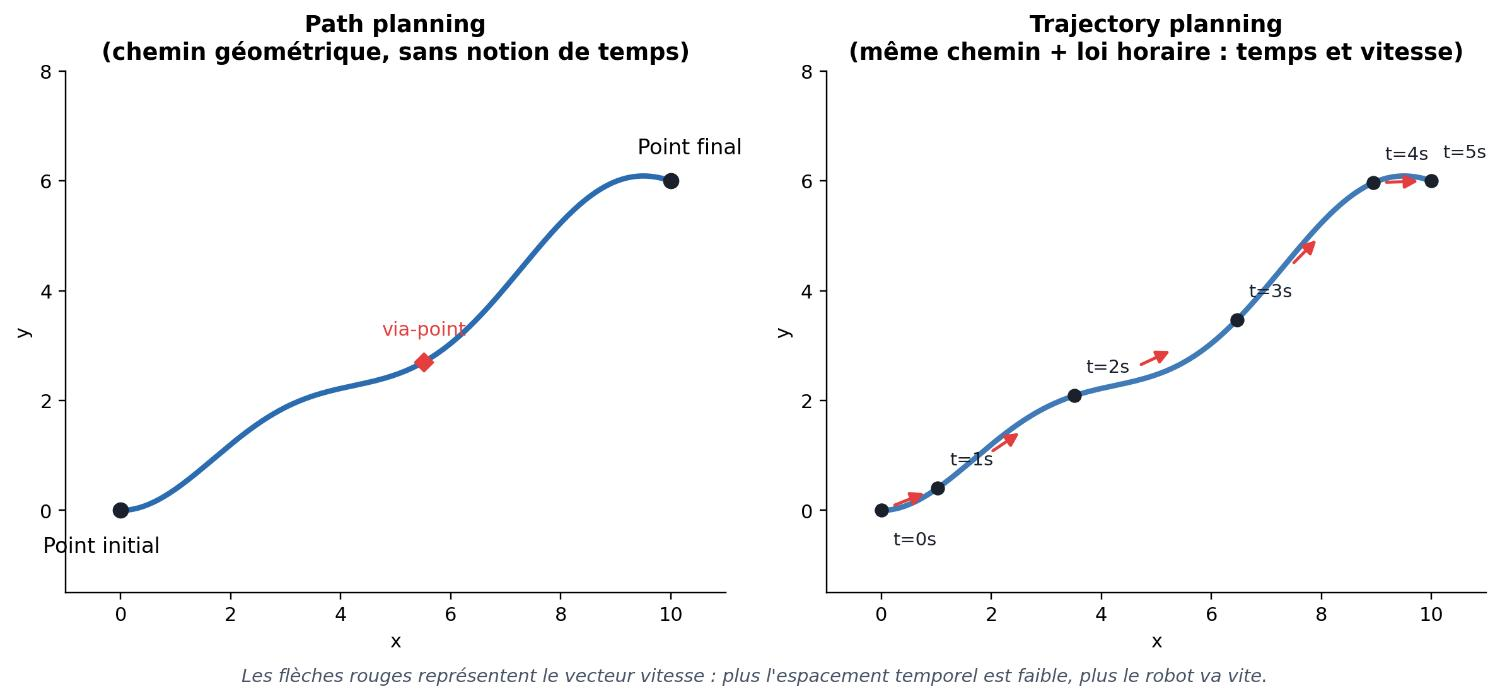
\includegraphics[width=0.88\textwidth]{path_vs_trajectory.png}
\caption{Comparaison chemin vs trajectoire}
\label{fig:path_vs_traj}
\end{figure}

\subsection{Faisabilité cinématique et dynamique}

La séparation entre path et trajectory planning permet de traiter la faisabilité du mouvement à deux niveaux complémentaires.

\textbf{Au niveau du path planning}, c'est purement géométrique : le chemin existe-t-il, et est-il admissible ? Cela implique de vérifier que le chemin ne traverse pas d'obstacles, qu'il respecte les limites de l'espace de travail, et qu'il est compatible avec la cinématique du mécanisme.

\textbf{Au niveau du trajectory planning}, cela devient temporelle et dynamique : le robot peut-il parcourir ce chemin dans les temps, sans dépasser les limites de vitesse et d'accélération de ses actionneurs, sans générer de vibrations excessives, et sans violer les contraintes dynamiques du système ? Les algorithmes de planification de trajectoire sont classiquement nommés selon la fonction qu'ils optimisent : \textbf{temps minimal}, \textbf{énergie minimale} ou \textbf{jerk minimal} \cite{gasparetto2015}.

\section{Génération de chemin}

La génération de chemin consiste à déterminer la courbe géométrique que le robot doit suivre, indépendamment de la considération temporelle. Selon la nature de la mission, deux grandes familles de problèmes se distinguent : la \textbf{couverture complète} d'une zone (Coverage Path Planning, CPP), où le robot doit passer par tous les points d'une région, et la \textbf{tournée de points discrets} (TSP, VRP), où il s'agit de visiter un ensemble fini de cibles selon un ordre. À ces deux familles s'ajoutent les algorithmes de recherche sur graphe ou par échantillonnage, mobilisés lorsque l'environnement est encombré d'obstacles \cite{gasparetto2015}.

\subsection{Couverture complète (CPP)}

La planification de chemin pour couverture complète a pour objectif de générer un chemin passant par \textbf{tous les points} d'une zone, sans distinction. Ce problème se rencontre dans plusieurs applications : nettoyage robotisé, cartographie, surveillance agricole, inspection de surfaces \cite{choset1998}.

\begin{figure}[H]
\centering
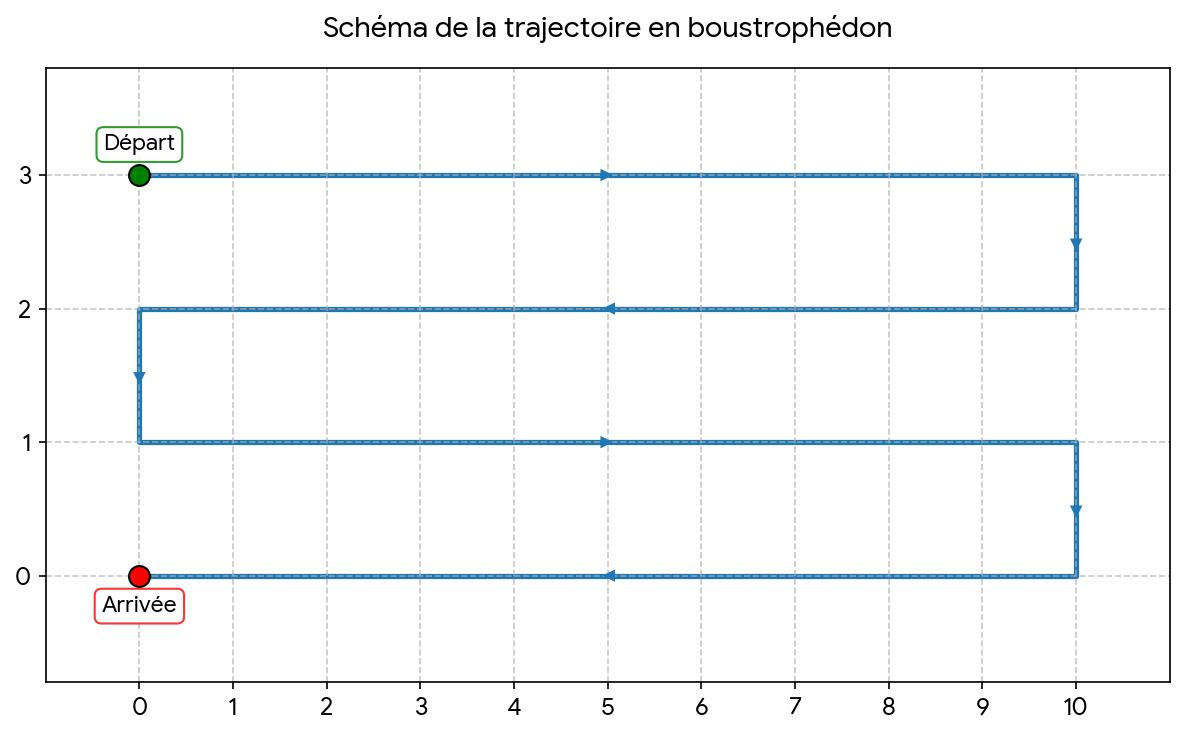
\includegraphics[width=0.85\textwidth]{boustrophedon.png}
\caption{Balayage boustrophédon}
\label{fig:boustrophedon}
\end{figure}

La méthode la plus établie demeure la \textbf{décomposition cellulaire boustrophédon} (Boustrophedon Cellular Decomposition, BCD), introduite par Choset et Pignon \cite{choset1998}. Son principe consiste à découper la zone à couvrir en \textbf{cellules convexes}, à l'aide de lignes verticales passant par les sommets des obstacles. Chaque cellule est ensuite balayée par des mouvements de va-et-vient parallèles d'où le terme « boustrophédon », qui désigne le mouvement du bœuf labourant un champ en effectuant des allers-retours successifs. Les cellules sont enfin reliées entre elles par un graphe d'adjacence, et un algorithme de parcours détermine l'ordre de visite optimal \cite{choset1998}.

\begin{figure}[H]
\centering
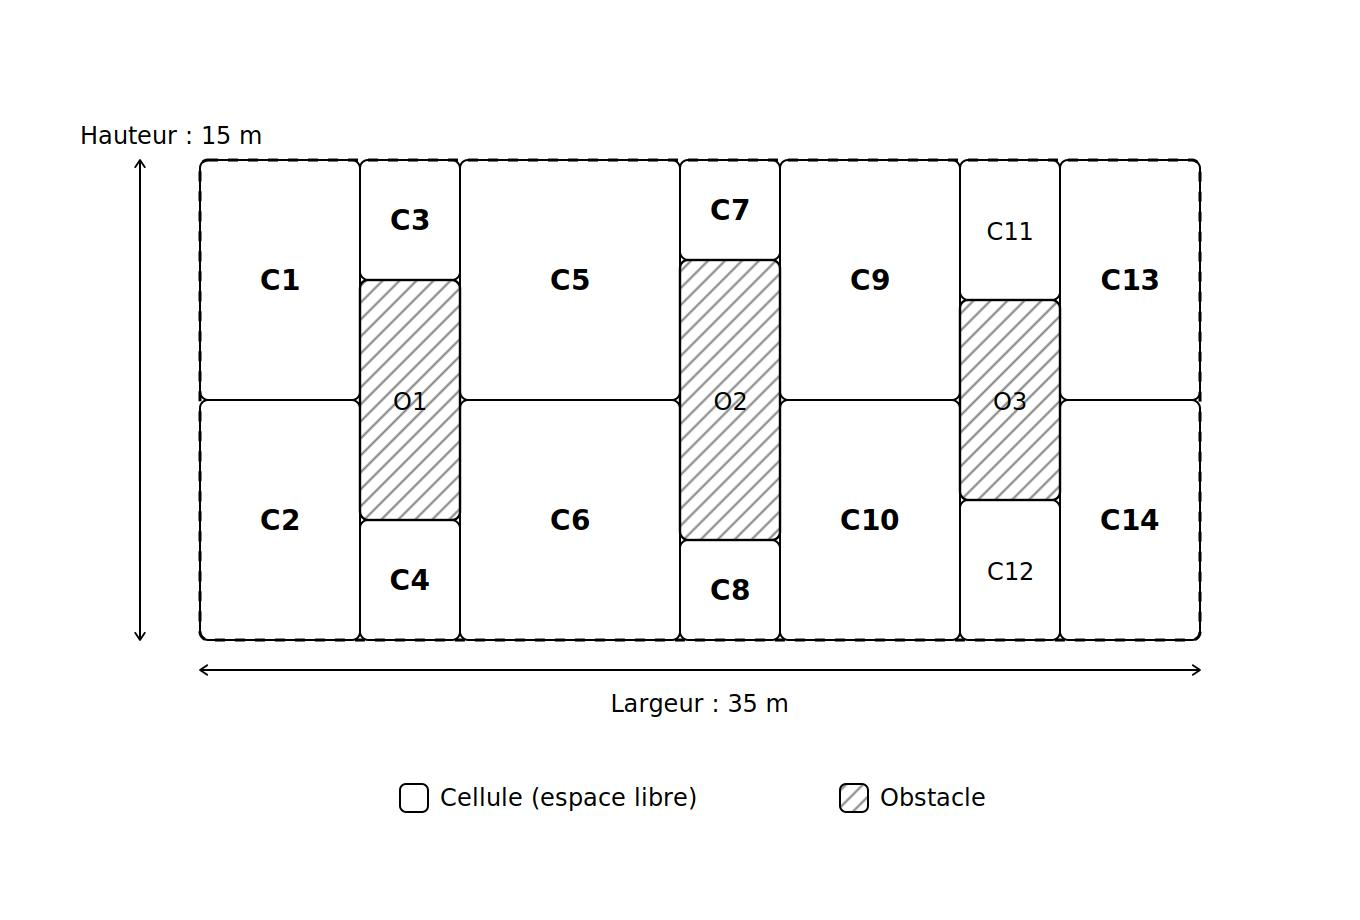
\includegraphics[width=0.90\textwidth]{decomposition_cellulaire.png}
\caption{Décomposition cellulaire (BCD)}
\label{fig:decomp_cell}
\end{figure}

Cette méthode garantit une couverture \textbf{complète} et \textbf{sans recouvrement inutile}, à condition que la zone soit plane et que les obstacles soient connus. Elle est particulièrement adaptée aux environnements structurés et de grande taille, tels que les parcelles agricoles \cite{choset1998}.

D'autres approches existent, comme les \textbf{trajectoires en spirale}, adaptées aux zones sans obstacle, et les \textbf{méthodes par champs de potentiel}. Le choix de la méthode dépend de la géométrie de la zone, de la présence d'obstacles et du critère d'optimisation retenu (temps et simplicité du chemin).

\subsection{Tournée de points discrets (TSP, VRP)}

Lorsque la mission ne consiste pas à couvrir une zone continue mais à \textbf{visiter un ensemble fini de points}, le problème se ramène à une tournée. Le cas le plus élémentaire est le \textbf{problème du voyageur de commerce} (Traveling Salesman Problem, TSP), qui consiste à déterminer l'ordre de visite de $N$ points minimisant la distance totale parcourue, avec retour au point de départ \cite{gasparetto2015}.

\begin{figure}[H]
\centering
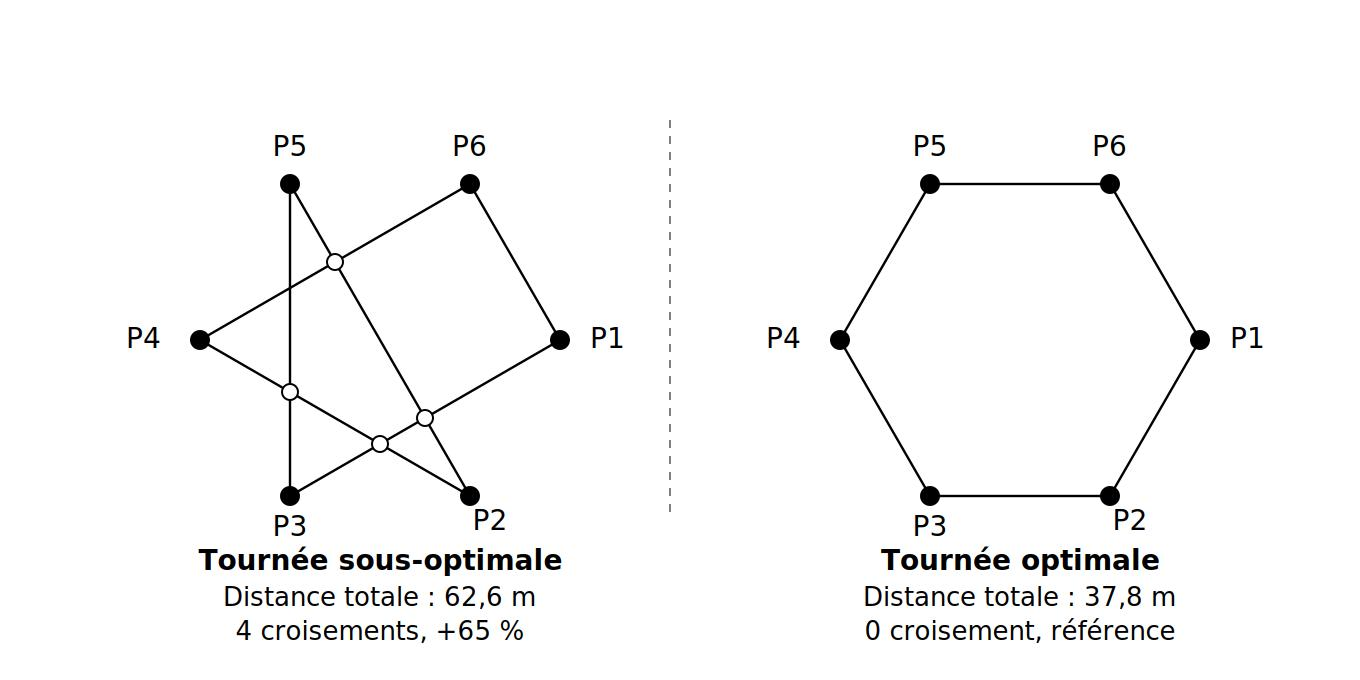
\includegraphics[width=0.88\textwidth]{tsp.png}
\caption{Tournées TSP : sous-optimale vs optimale}
\label{fig:tsp}
\end{figure}

Le TSP constitue un problème \textbf{NP-difficile} : le nombre de permutations possibles croît en $N!$, rendant toute résolution exacte impraticable au-delà d'une vingtaine de points. Pour des instances de taille supérieure, on utilise des \textbf{heuristiques} (plus proche voisin, insertion, 2-opt) ou à des \textbf{métaheuristiques} (algorithmes génétiques, recuit simulé), permettant d'obtenir des solutions proches de l'optimum dans un temps de calcul raisonnable \cite{gasparetto2015}.

Le \textbf{problème de tournée de véhicules} (Vehicle Routing Problem, VRP) constitue une généralisation du TSP à plusieurs véhicules desservant un ensemble de clients. Sa variante avec fenêtres temporelles (VRPTW) impose que chaque client soit visité dans un intervalle de temps donné. Ces problèmes, également NP-difficiles, se rencontrent en logistique et en planification de tournées \cite{gasparetto2015}.

\subsection{Algorithmes de graphe et échantillonnage}

Lorsque l'environnement est encombré d'obstacles, la génération de chemin se ramène généralement à une \textbf{recherche sur graphe}. L'espace libre est discrétisé en un ensemble de nœuds connectés par des arêtes, et un algorithme de plus court chemin détermine la séquence optimale.

Les algorithmes classiques comprennent :
\begin{itemize}
\item \textbf{Dijkstra} : détermine le plus court chemin d'un nœud source vers l'ensemble des autres nœuds, en présence de poids positifs.
\item \textbf{A*} : variante de Dijkstra guidée par une fonction heuristique, plus efficace en pratique.
\item \textbf{Floyd-Warshall} : calcule les plus courts chemins entre toutes les paires de nœuds, pour un coût de $O(n^3)$.
\end{itemize}

Ces algorithmes sont déterministes et garantissent l'optimalité, mais leur complexité dépend directement de la finesse de la discrétisation retenue. Une grille trop fine entraîne une explosion du temps de calcul ; une grille trop grossière produit des chemins en escalier \cite{gasparetto2015}.

Pour les environnements de grande dimension, les \textbf{méthodes d'échantillonnage probabiliste} sont généralement privilégiées :
\begin{itemize}
\item \textbf{RRT} (Rapidly-exploring Random Tree) : construit un arbre en explorant aléatoirement l'espace jusqu'à atteindre la cible.
\item \textbf{PRM} (Probabilistic Roadmap) : construit un graphe de routes par échantillonnage de l'espace libre, sur lequel un chemin est ensuite recherché.
\end{itemize}

\begin{figure}[H]
\centering
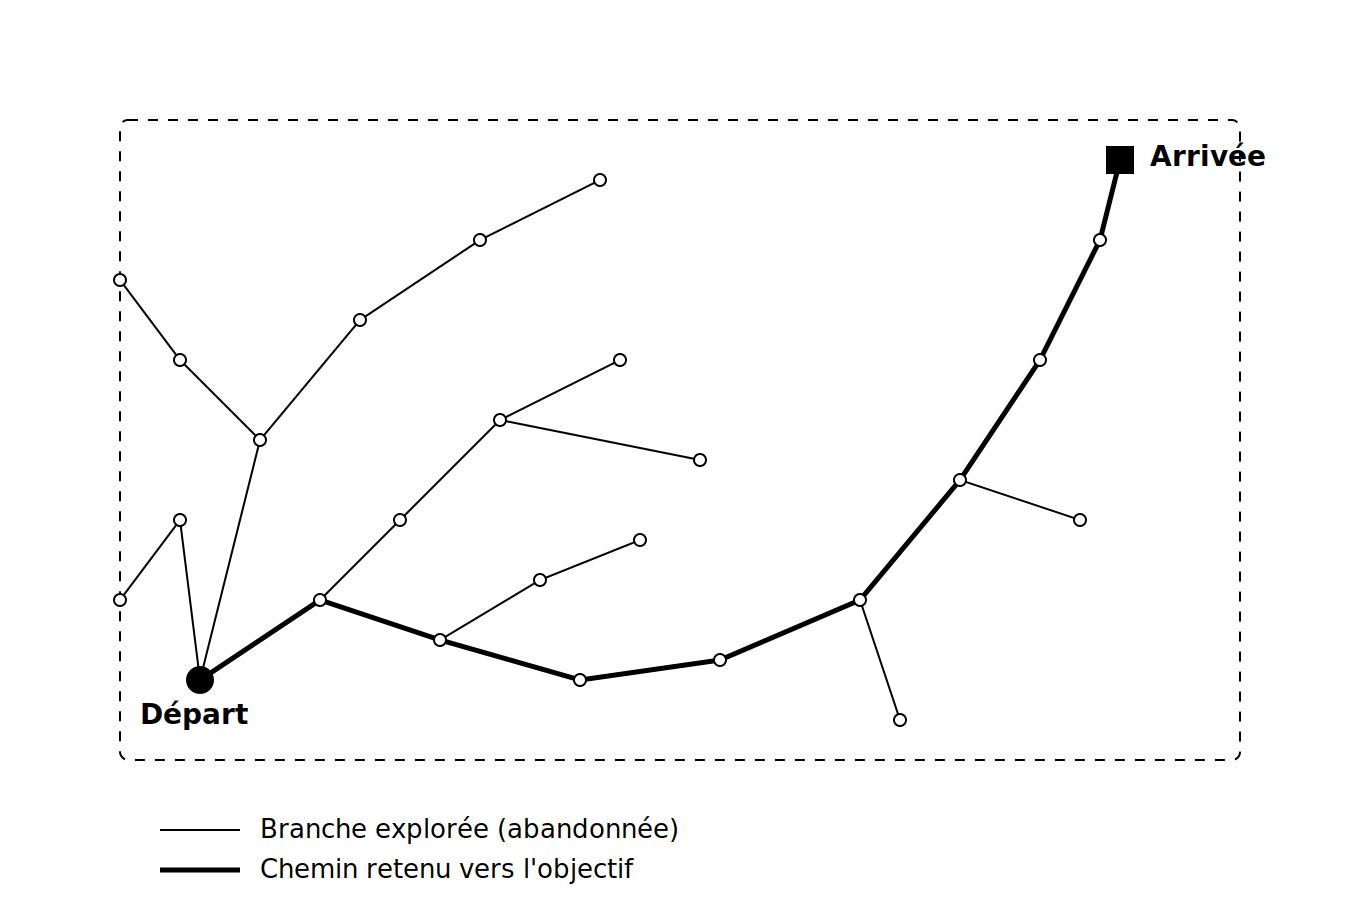
\includegraphics[width=0.80\textwidth]{rrt.png}
\caption{Principe de l'algorithme RRT}
\label{fig:rrt}
\end{figure}

Ces méthodes sont \textbf{probabilistes} : elles convergent vers une solution avec une probabilité croissante, sans garantir l'optimalité. Elles sont adaptées aux robots présentant un grand nombre de degrés de liberté, mais s'avèrent moins efficaces que les méthodes déterministes dans des espaces simples et structurés \cite{gasparetto2015}.

Le tableau ci-dessous résume les caractéristiques des principales familles de méthodes.

\begin{table}[H]
\centering
\caption{Tableau comparatif des méthodes de génération de chemin}
\label{tab:methodes_chemin}
\footnotesize
\begin{tabular}{|>{\raggedright\arraybackslash}p{2.5cm}|>{\raggedright\arraybackslash}p{2.3cm}|>{\raggedright\arraybackslash}p{2.1cm}|>{\raggedright\arraybackslash}p{2.3cm}|>{\raggedright\arraybackslash}p{2.9cm}|}
\hline
\textbf{Méthode} & \textbf{Type de problème} & \textbf{Optimalité} & \textbf{Complexité} & \textbf{Adaptée à} \\
\hline
Boustrophédon (BCD) & Couverture complète & Complète & Modérée & Zones structurées sans obstacle complexe \\
\hline
Spirale & Couverture complète & Complète & Faible & Zones convexes sans obstacle \\
\hline
TSP (exact) & Tournée de points & Optimale & $O(N!)$ explose & Très petits ensembles ($N < 20$) \\
\hline
TSP (heuristique) & Tournée de points & Proche de l'optimum & $O(N^2)$ à $O(N^3)$ & Grands ensembles \\
\hline
Dijkstra / A* & Graphe discret & Optimale & $O(n \log n)$ & Environnements discrets modérés \\
\hline
RRT / PRM & Espace continu & Probabiliste & Variable & Environnements complexes, grande dimension \\
\hline
\end{tabular}
\end{table}

\textbf{Remarque :} le choix d'une méthode dépend de la nature de la tâche (couverture ou visite de points), de la taille de l'espace considéré, de la présence d'obstacles et du compromis entre optimalité et temps de calcul. Pour une zone structurée et sans obstacle, la \textbf{décomposition boustrophédon} \cite{choset1998} constitue la méthode la plus simple et la plus robuste pour assurer une couverture complète. Pour la visite de points précis, une \textbf{heuristique de type plus proche voisin} offre un compromis satisfaisant entre qualité de solution et temps de calcul. Les algorithmes de graphe et d'échantillonnage sont réservés aux environnements encombrés ou de grande dimension \cite{gasparetto2015}.

\section{Lissage de trajectoire}

Une fois le chemin géométrique déterminé (section 2.2), il faut définir comment le robot va le parcourir dans le temps. Cette étape, appelée \textit{trajectory planning}, consiste à associer à chaque point du chemin un instant de passage, une vitesse et une accélération. Le choix de la méthode d'interpolation conditionne directement la douceur du mouvement, les sollicitations mécaniques et la qualité du suivi \cite{gasparetto2015}.

\begin{figure}[H]
\centering
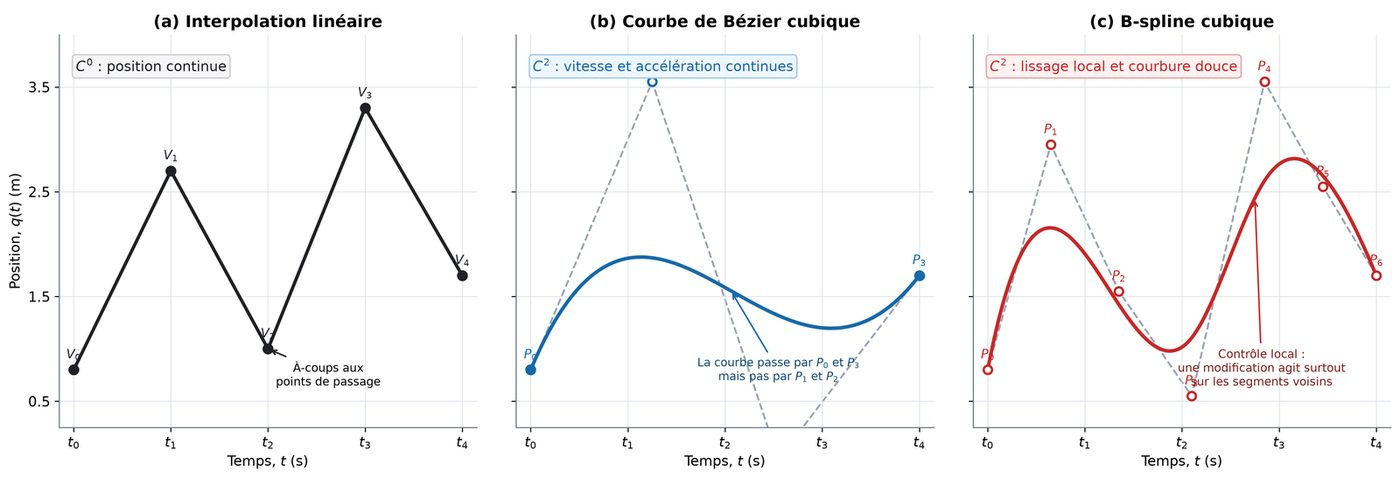
\includegraphics[width=0.98\textwidth]{lissage.jpg}
\caption{Comparaison des méthodes de lissage}
\label{fig:lissage}
\end{figure}

\begin{itemize}
\item La méthode la plus simple consiste à relier les points de passage par des \textbf{segments de droite}, en imposant une vitesse constante sur chaque segment. Cette approche, dite \textbf{interpolation linéaire}, est simple à mettre en œuvre.

Cependant, elle possède \textbf{deux limites majeures} \cite{gasparetto2015} :
\begin{itemize}
\item \textbf{Discontinuité de vitesse aux points de passage.} Lorsque le robot change de segment, sa vitesse passe brutalement d'une valeur à une autre, ce qui se traduit par un \textbf{à-coup} mécanique. Cette discontinuité est de classe $C^0$ (continuité de position seulement), insuffisante pour un mouvement fluide.
\item \textbf{Discontinuité d'accélération.} Aux extrémités de chaque segment, l'accélération est théoriquement infinie. En pratique, cela se traduit par des pics de couple sur les actionneurs, des vibrations et une usure prématurée de la mécanique.
\end{itemize}

Ces défauts sont particulièrement pénalisants pour les robots à structure flexible, comme les robots à câbles, où les à-coups provoquent les modes vibratoires et dégradent la précision. Pour obtenir un mouvement fluide, il faut donc utiliser des \textbf{courbes lisses} garantissant la continuité de la vitesse et, idéalement, de l'accélération.
\end{itemize}

\subsection{Courbes de Bézier et B-splines}

Les \textbf{courbes de Bézier} et les \textbf{B-splines} sont les deux familles de courbes paramétriques les plus utilisées en robotique pour le lissage de trajectoire \cite{gasparetto2015}.

Une \textbf{courbe de Bézier} de degré $n$ est définie par $n+1$ points de contrôle. Elle passe par le premier et le dernier point de contrôle, mais pas par les points intermédiaires. Sa forme est entièrement déterminée par le polygone de contrôle, ce qui la rend facile à manipuler. Le degré de continuité dépend du degré du polynôme : une courbe de Bézier cubique (degré 3) assure une continuité $C^2$ (position, vitesse et accélération continues).

Les \textbf{B-splines} généralisent les courbes de Bézier en les assemblant par morceaux. Elles offrent deux avantages majeurs :
\begin{itemize}
\item \textbf{Contrôle local} : modifier un point de contrôle n'affecte que les segments voisins, contrairement aux courbes de Bézier où tout est couplé.
\item \textbf{Degré de continuité paramétrable} : une B-spline de degré $k$ assure une continuité $C^{k-1}$. On utilise couramment des B-splines cubiques ($C^2$) ou quintiques ($C^3$, continuité du jerk).
\end{itemize}

Le tableau ci-dessous résume les niveaux de continuité obtenus selon la méthode :

\begin{table}[H]
\centering
\caption{Niveaux de continuité selon la méthode de lissage}
\label{tab:continuite}
\begin{tabular}{|l|c|c|l|}
\hline
\textbf{Méthode} & \textbf{Continuité} & \textbf{Degré} & \textbf{Passage exact par les points} \\
\hline
Interpolation linéaire & $C^0$ & 1 & Oui \\
\hline
Courbe de Bézier cubique & $C^2$ & 3 & Non (points de contrôle) \\
\hline
B-spline cubique & $C^2$ & 3 & Non (approximation) \\
\hline
B-spline quintique & $C^3$ & 5 & Non (approximation) \\
\hline
\end{tabular}
\end{table}

\subsection{Le profil LSPB (Linear Segments with Parabolic Blends)}

Les B-splines et les courbes de Bézier sont particulièrement adaptées aux trajectoires \textbf{continues}, où le robot ne s'arrête pas entre les points de passage. Cependant, dans de nombreuses applications, le robot doit \textbf{s'arrêter complètement} à chaque point (par exemple, pour effectuer une mesure, une prise de vue ou une opération de précision). Dans ce cas, le lissage par B-spline perd une partie de son intérêt : comme le robot s'arrête, il n'y a pas d'angle vif à lisser, et la continuité de la vitesse est naturellement assurée (elle est nulle à chaque point).

La solution retenue dans ce cas est le \textbf{profil de vitesse trapézoïdal}, également appelé \textbf{LSPB} (Linear Segments with Parabolic Blends) \cite{lspb}. Ce profil se compose de trois phases :
\begin{enumerate}
\item \textbf{Phase d'accélération} : la vitesse croît linéairement (accélération constante) jusqu'à atteindre la vitesse de croisière.
\item \textbf{Phase de croisière} : la vitesse reste constante à sa valeur maximale.
\item \textbf{Phase de décélération} : la vitesse décroît linéairement jusqu'à zéro.
\end{enumerate}

Si le segment est trop court pour atteindre la vitesse maximale, le profil devient \textbf{triangulaire} : les phases d'accélération et de décélération se rejoignent sans phase de croisière.

\begin{figure}[H]
\centering
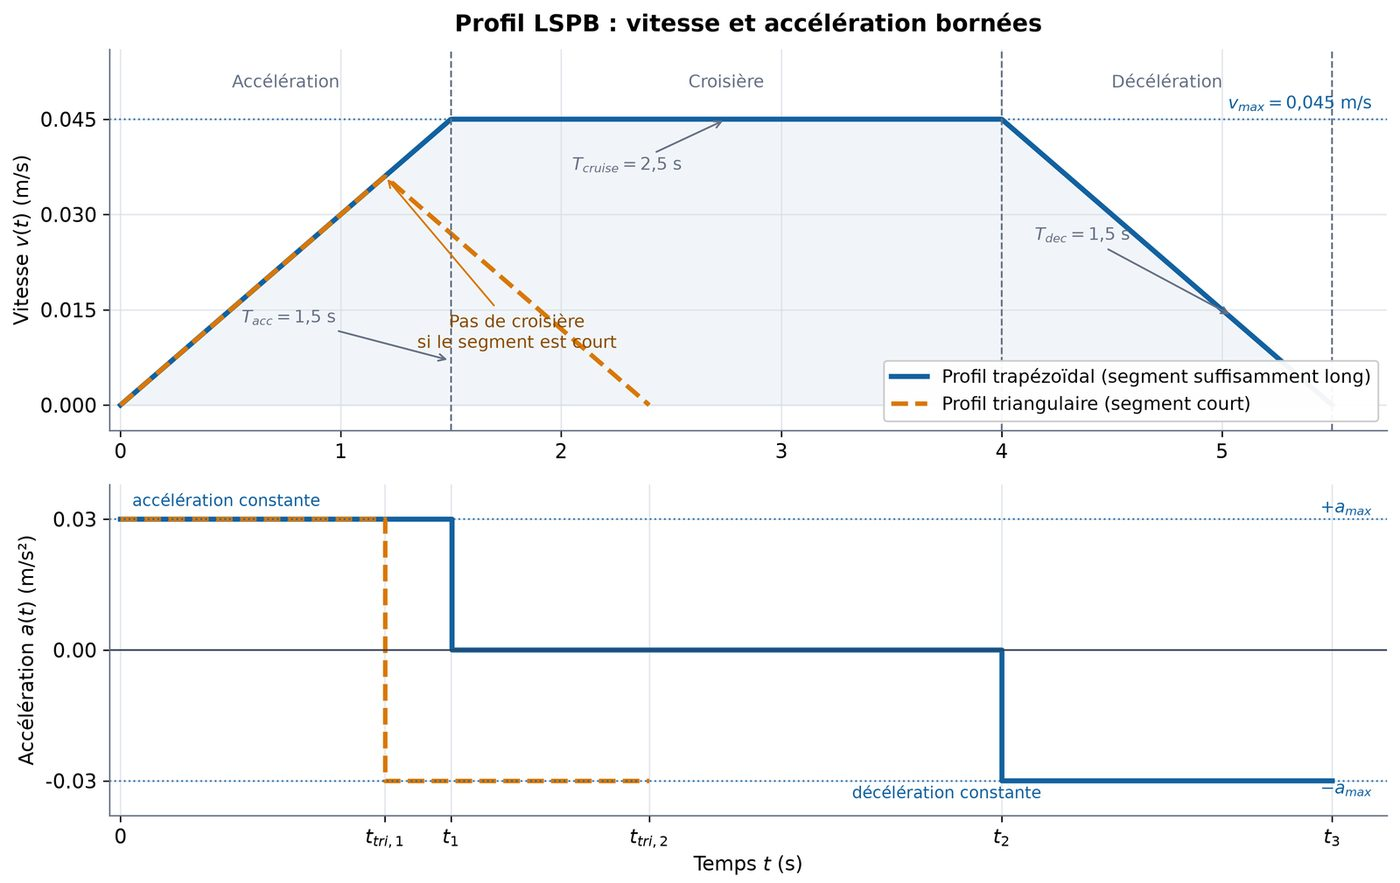
\includegraphics[width=0.95\textwidth]{lspb.jpg}
\caption{Profil de vitesse LSPB}
\label{fig:lspb}
\end{figure}

Le profil LSPB présente plusieurs avantages pour les trajectoires point-à-point \cite{lspb} :
\begin{itemize}
\item \textbf{Continuité de la vitesse} : la vitesse est nulle au départ et à l'arrivée, et continue pendant tout le mouvement.
\item \textbf{Accélération bornée} : l'accélération reste constante (ou nulle) sur chaque phase, ce qui évite les pics de couple.
\item \textbf{Implémentation simple} : le calcul des instants de transition est analytique, sans résolution numérique.
\item \textbf{Passage exact par les points} : contrairement aux B-splines, le robot passe exactement par chaque point de passage, ce qui est essentiel pour les applications de mesure.
\end{itemize}

En résumé, le \textbf{profil LSPB} constitue un bon compromis entre simplicité, continuité de la vitesse et respect des contraintes cinématiques. Il est particulièrement adapté aux trajectoires \textbf{point-à-point avec arrêt complet}, où les B-splines n'apportent pas de bénéfice significatif.

\section{Contraintes de planification}

La génération d'un chemin (section 2.2) et son lissage (section 2.3) ne suffisent pas à garantir qu'une trajectoire est réalisable. La planification doit en effet intégrer un ensemble de contraintes qui conditionnent le mouvement du robot. Ces contraintes se répartissent en quatre familles : mécaniques, cinématiques, visibilité et stabilité.

\subsection{Contraintes mécaniques}

Dans un robot parallèle à câbles, la contrainte mécanique fondamentale est l'\textbf{unilatéralité des câbles} : un câble ne peut transmettre qu'un effort de traction, jamais de poussée. Par conséquent, la tension dans chaque câble doit rester strictement positive à tout instant. En pratique, on impose une tension minimale $T_{\min}$ pour garantir que les câbles ne se détendent pas sous l'effet des perturbations, et une tension maximale $T_{\max}$ pour ne pas dépasser la capacité des moteurs ou la résistance des câbles.

Le respect simultané de ces bornes définit l'\textbf{espace de travail faisable en effort} (Wrench-Feasible Workspace, WFW), déjà introduit en section 1.5.4. Gouttefarde et al. \cite{gouttefarde2011} ont montré que le WFW peut être déterminé par une analyse par intervalles, qui garantit l'existence d'une distribution de tensions admissible pour une pose donnée. Une trajectoire n'est réalisable que si elle reste \textbf{intégralement incluse} dans le WFW. La planification doit donc vérifier, pour chaque point de la trajectoire, que le problème d'équilibre statique admet une solution en tensions respectant les bornes.



\subsection{Contraintes cinématiques}

Les contraintes cinématiques portent sur les \textbf{vitesses} et \textbf{accélérations} maximales que les actionneurs peuvent fournir, ainsi que sur le \textbf{jerk} (dérivée de l'accélération) lorsque la continuité de l'accélération est requise \cite{gasparetto2015}.

Pour un robot à câbles, ces contraintes se traduisent directement sur les vitesses de déroulement des câbles : $\dot{l}_i \leq \dot{l}_{\max}$ et $\ddot{l}_i \leq \ddot{l}_{\max}$. Ces limites sont imposées par la vitesse maximale des moteurs et par la capacité des enrouleurs à accélérer sans décrochage. La planification de trajectoire doit donc garantir que le profil de vitesse retenu (par exemple un profil LSPB, section 2.3.3) respecte ces bornes sur l'ensemble du chemin.

\subsection{Contraintes de visibilité}

Lorsque le robot embarque un capteur (caméra, lidar), la planification doit également respecter des contraintes de \textbf{visibilité} : le capteur doit être orienté vers la cible, à une distance et un angle compatible avec ses caractéristiques (champ de vision, résolution, profondeur de champ). Ces contraintes se traduisent par des exigences sur l'\textbf{orientation} de la plateforme et sur sa \textbf{position relative} par rapport aux points d'intérêt.

Dans le cas d'un robot à câbles, ces contraintes sont particulièrement délicates car l'orientation de la plateforme est souvent contrainte par la géométrie des câbles. Si l'orientation doit être pilotée, il faut vérifier que le WFW reste non vide pour la pose complète (position + orientation). Si l'orientation est fixe (comme dans le cas d'une plateforme en translation pure), les contraintes de visibilité se réduisent à des contraintes de position.

\subsection{Contraintes de stabilité}

Les robots à câbles sont sujets aux \textbf{vibrations}, en raison de la faible rigidité des câbles et de leur amortissement naturel très faible. Ces vibrations dégradent la précision du positionnement et augmentent le \textbf{temps d'établissement} : le temps nécessaire pour que la plateforme se stabilise à une position donnée après un mouvement.

Khayour \cite{khayour2022} souligne que la flexibilité des câbles réduit la bande passante des efforts qu'ils peuvent transmettre, ce qui limite la capacité à amortir les vibrations et à suivre des trajectoires dynamiques. Pour garantir la stabilité, la planification doit donc éviter les \textbf{à-coups} (jerk élevé) et prévoir des \textbf{temps d'arrêt} suffisants à chaque point de mesure ou d'opération. Ces temps d'arrêt, appelés temps de stabilisation, dépendent des caractéristiques vibratoires du système (fréquences propres, amortissement) et des exigences de précision.

\begin{figure}[H]
\centering
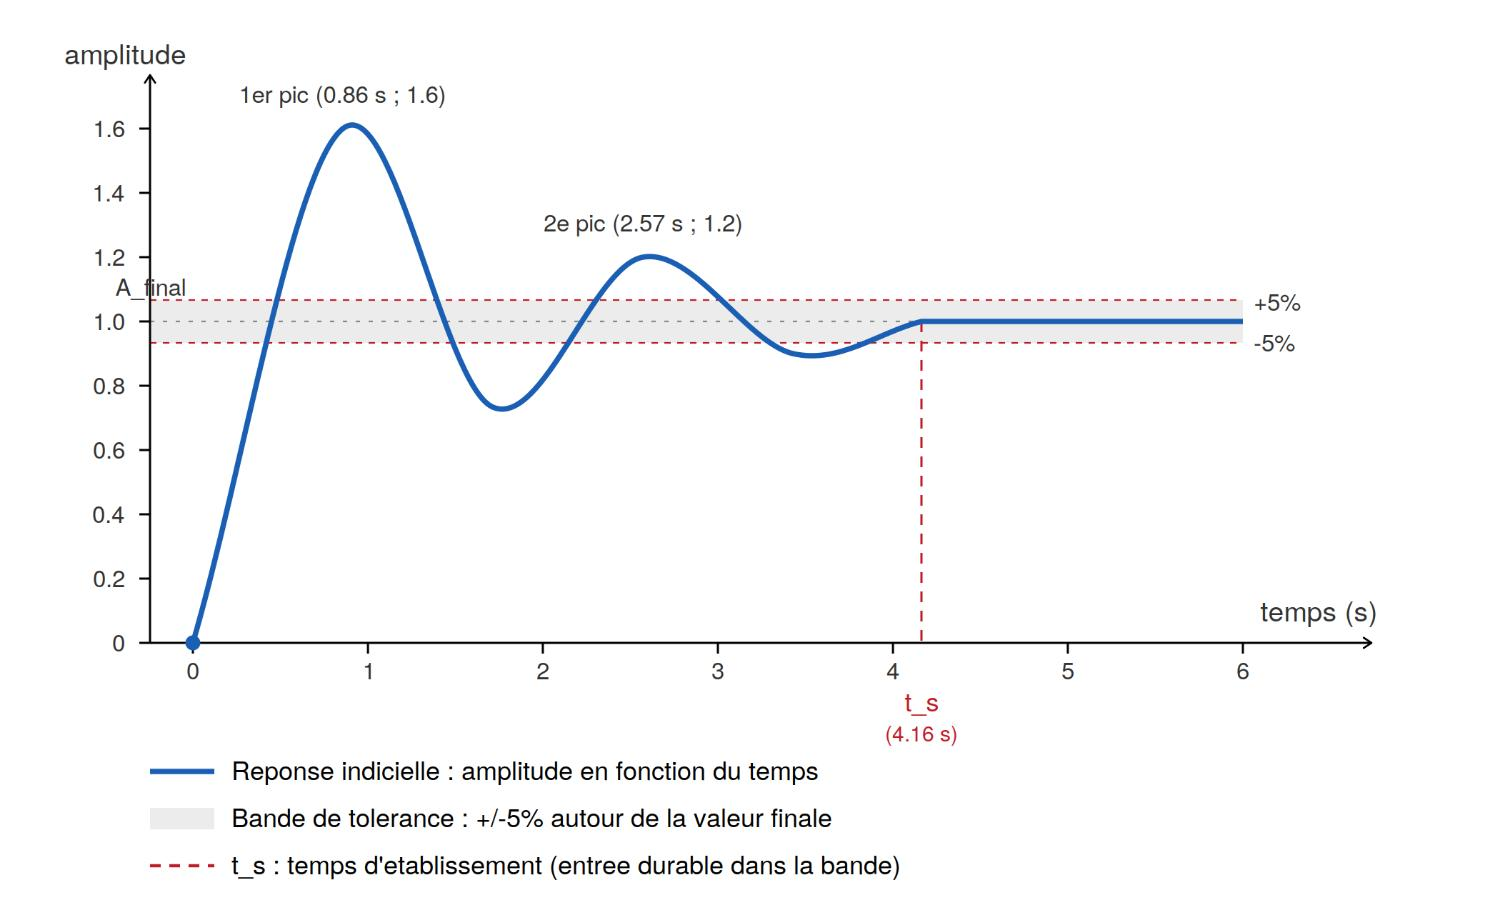
\includegraphics[width=0.72\textwidth]{systeme_vibratoire.png}
\caption{Réponse indicielle et temps d'établissement}
\label{fig:vibratoire}
\end{figure}

\section{Cadre d'optimisation}

La génération de chemin (section 2.2) et le lissage de trajectoire (section 2.3) produisent une trajectoire \textit{faisable}. Cependant, il existe généralement une \textbf{infinité de trajectoires faisables} pour une même tâche. Le cadre d'optimisation a pour objectif de sélectionner, parmi ces solutions, celle qui minimise (ou maximise) un ou plusieurs \textbf{critères de performance} tout en respectant les contraintes (section 2.4).

\begin{figure}[H]
\centering
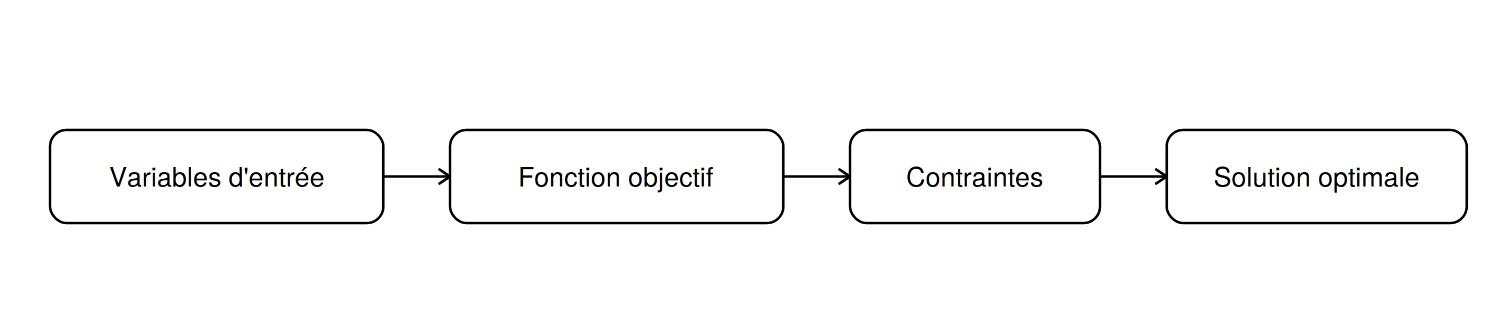
\includegraphics[width=0.80\textwidth]{probleme_optimisation.png}
\caption{Structure d'un problème d'optimisation}
\label{fig:optimisation}
\end{figure}

\subsection{Formulation du problème}

Un problème d'optimisation se formalise par trois éléments \cite{gasparetto2015} :
\begin{itemize}
\item \textbf{Variables de décision} : les paramètres (ordre de visite, instants de passage, paramètres du profil de vitesse, etc.).
\item \textbf{Fonction objectif} : la quantité à minimiser ou maximiser (temps, énergie, jerk, etc.).
\item \textbf{Contraintes} : les limitations à respecter (bornes de tension, limites de vitesse, contraintes de visibilité, etc.).
\end{itemize}

Mathématiquement :
\begin{equation}
\min_{\mathbf{x}} \quad f(\mathbf{x}) \quad \text{sous contraintes} \quad g_i(\mathbf{x}) \leq 0, \quad h_j(\mathbf{x}) = 0
\label{eq:optimisation}
\end{equation}
où
\begin{itemize}
\item $\mathbf{x}$ est le vecteur des variables de décision,
\item $f$ la fonction objectif,
\item $g_i$ les contraintes d'inégalité et
\item $h_j$ les contraintes d'égalité.
\end{itemize}

La difficulté du problème dépend de la nature de $f$ (linéaire, non linéaire, convexe) et des contraintes \cite{gasparetto2015}.

\subsection{Optimisation mono et multi-objectif}

Lorsqu'un seul critère est optimisé, on parle d'\textbf{optimisation mono-objectif} : la solution est unique (ou appartient à un ensemble d'indifférence). Les méthodes classiques (gradient, programmation linéaire) s'appliquent directement.

Lorsque plusieurs critères \textbf{conflictuels} doivent être optimisés simultanément (par exemple, minimiser le temps \textit{et} l'énergie), on parle d'\textbf{optimisation multi-objectif}. Il n'existe alors généralement pas de solution unique, mais un ensemble de solutions \textbf{non dominées} appelé \textbf{front de Pareto} \cite{gasparetto2015}. Une solution $A$ domine une solution $B$ si $A$ est meilleure ou égale sur tous les objectifs, et strictement meilleure sur au moins un. Le front de Pareto représente le meilleur compromis possible entre les objectifs.

\begin{figure}[H]
\centering
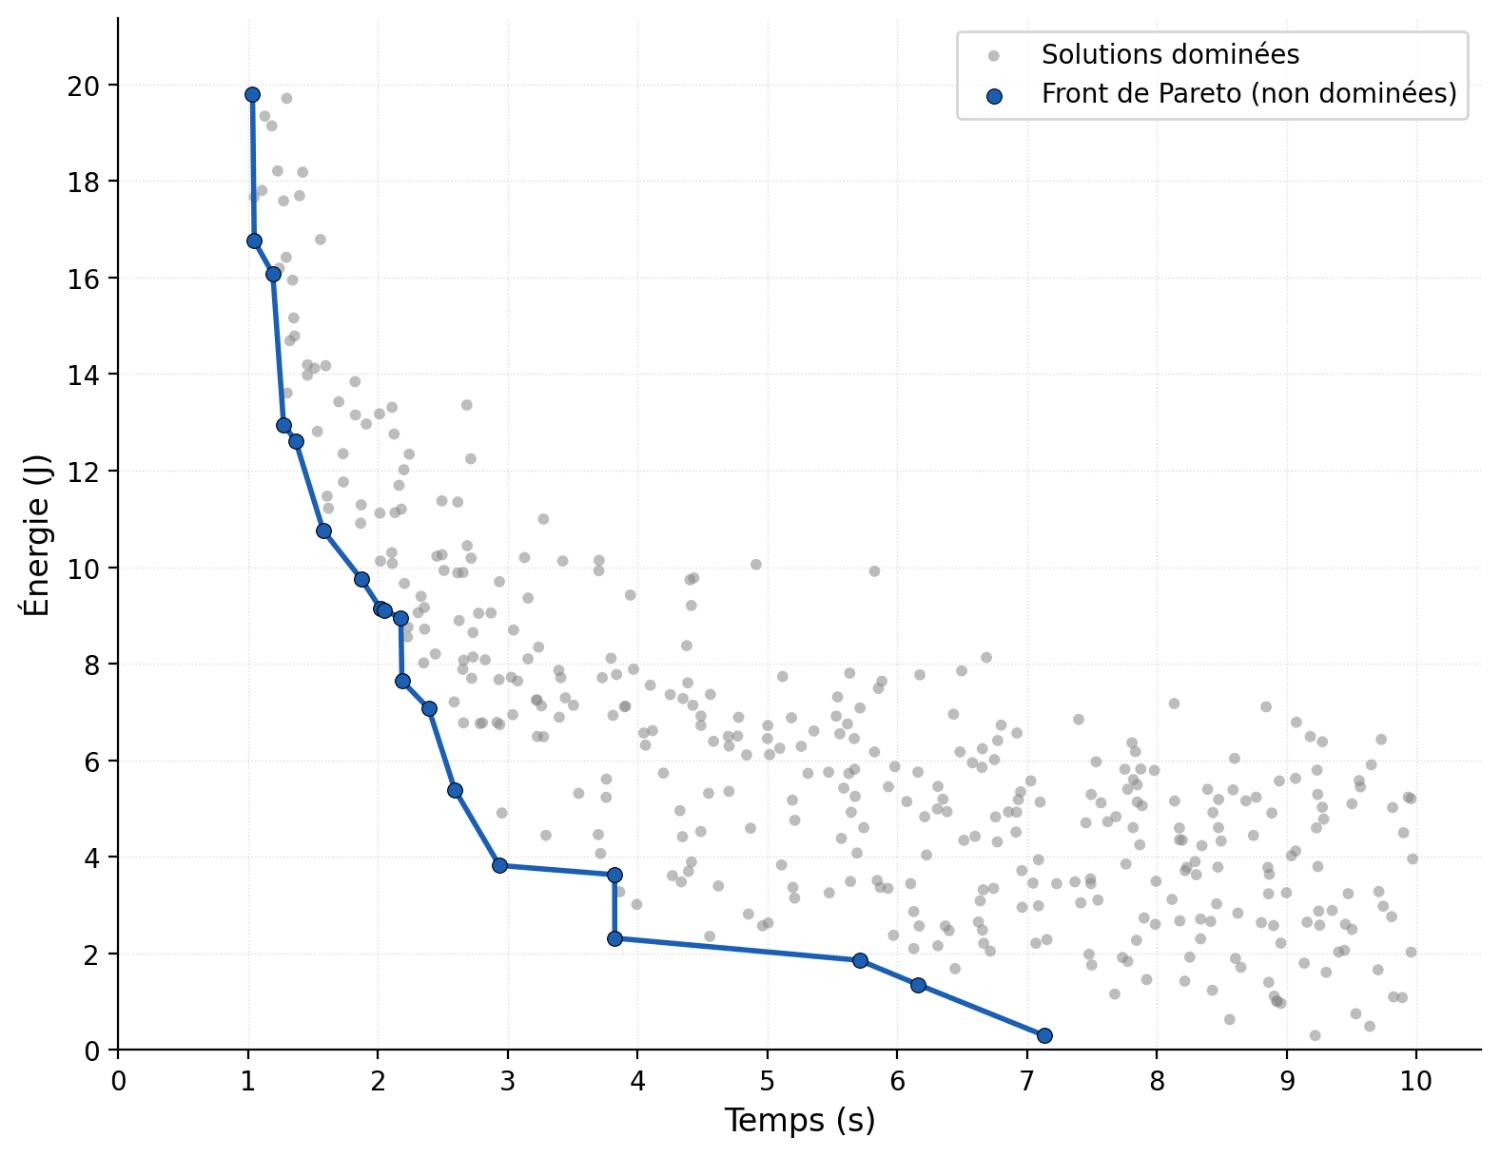
\includegraphics[width=0.72\textwidth]{front_pareto.png}
\caption{Front de Pareto (temps vs énergie)}
\label{fig:pareto}
\end{figure}

\subsection{Modèle énergétique}

Le \textbf{modèle énergétique} permet d'estimer la consommation d'énergie associée à une trajectoire. Pour un robot à câbles, l'énergie dépend principalement des tensions dans les câbles, des vitesses de déroulement, des accélérations et des pertes dans les moteurs \cite{gasparetto2015}, \cite{lspb}.

Un modèle simplifié consiste à intégrer la puissance mécanique sur la durée de la trajectoire :
\begin{equation}
E = \int_{0}^{T} \sum_{i=1}^{m} T_i(t) \, |\dot{l}_i(t)| \, dt
\label{eq:energie}
\end{equation}
où
\begin{itemize}
\item $T_i$ est la tension dans le câble $i$,
\item $\dot{l}_i$ sa vitesse de déroulement.
\end{itemize}

\subsection{Méthodes exactes}

Les \textbf{méthodes exactes} garantissent la solution optimale en un temps fini. Elles sont adaptées aux problèmes de petite taille ou de structure particulière \cite{gasparetto2015} : programmation linéaire (LP), programmation quadratique (QP), programmation dynamique, méthodes par branchement et bornes. Leur efficacité décroît rapidement lorsque le nombre de variables ou la non-linéarité augmentent. On recourt alors à des méthodes approchées.

\subsection{Métaheuristiques mono-objectif}

Les \textbf{métaheuristiques} sont des algorithmes d'optimisation de haut niveau, inspirés de phénomènes naturels, qui fournissent de bonnes solutions en un temps raisonnable sans garantir l'optimalité. Pour l'optimisation mono-objectif, les plus utilisées sont \cite{gasparetto2015} : recuit simulé, algorithmes génétiques (GA), optimisation par essaim particulaire (PSO), colonies de fourmis (ACO). Ces méthodes nécessitent un réglage de paramètres et peuvent converger vers des optimums locaux.

\subsection{Métaheuristiques multi-objectif}

Pour l'optimisation multi-objectif, les métaheuristiques doivent produire un \textbf{ensemble de solutions non dominées} (front de Pareto). Les algorithmes les plus utilisés sont \cite{gasparetto2015} : \textbf{NSGA-II}, \textbf{MOEA/D} et \textbf{MOPSO}. Parmi eux, NSGA-II \cite{deb2002} constitue un algorithme de référence pour les problèmes à deux ou trois objectifs. Sa robustesse, sa convergence rapide et sa capacité à maintenir un front bien réparti en font une méthode largement étudiée dans la littérature.

\subsubsection{Principe général du NSGA-II}

NSGA-II est un \textbf{algorithme génétique} : il fait évoluer une \textbf{population} d'individus (solutions candidates) au fil de \textbf{générations} successives, en appliquant les principes de sélection, croisement et mutation. Ce qui le distingue d'un algorithme génétique classique, c'est sa capacité à gérer \textbf{plusieurs objectifs simultanément} en classant les individus selon leur \textbf{dominance} et en préservant la \textbf{diversité} du front de Pareto \cite{deb2002}.

Un individu (ou chromosome) code une solution candidate. Selon la nature du problème, le codage peut être \textbf{réel} (paramètres continus), \textbf{par permutation} (ordre de visite) ou \textbf{binaire}.

\subsubsection{Étapes de l'algorithme}

\textbf{Étape 1 : Initialisation.}

Une population initiale de $N$ individus est générée aléatoirement. Chaque individu est évalué selon les $M$ objectifs, ce qui donne un vecteur de coûts $(f_1, f_2, \ldots, f_M)$.

\begin{figure}[!htbp]
\centering
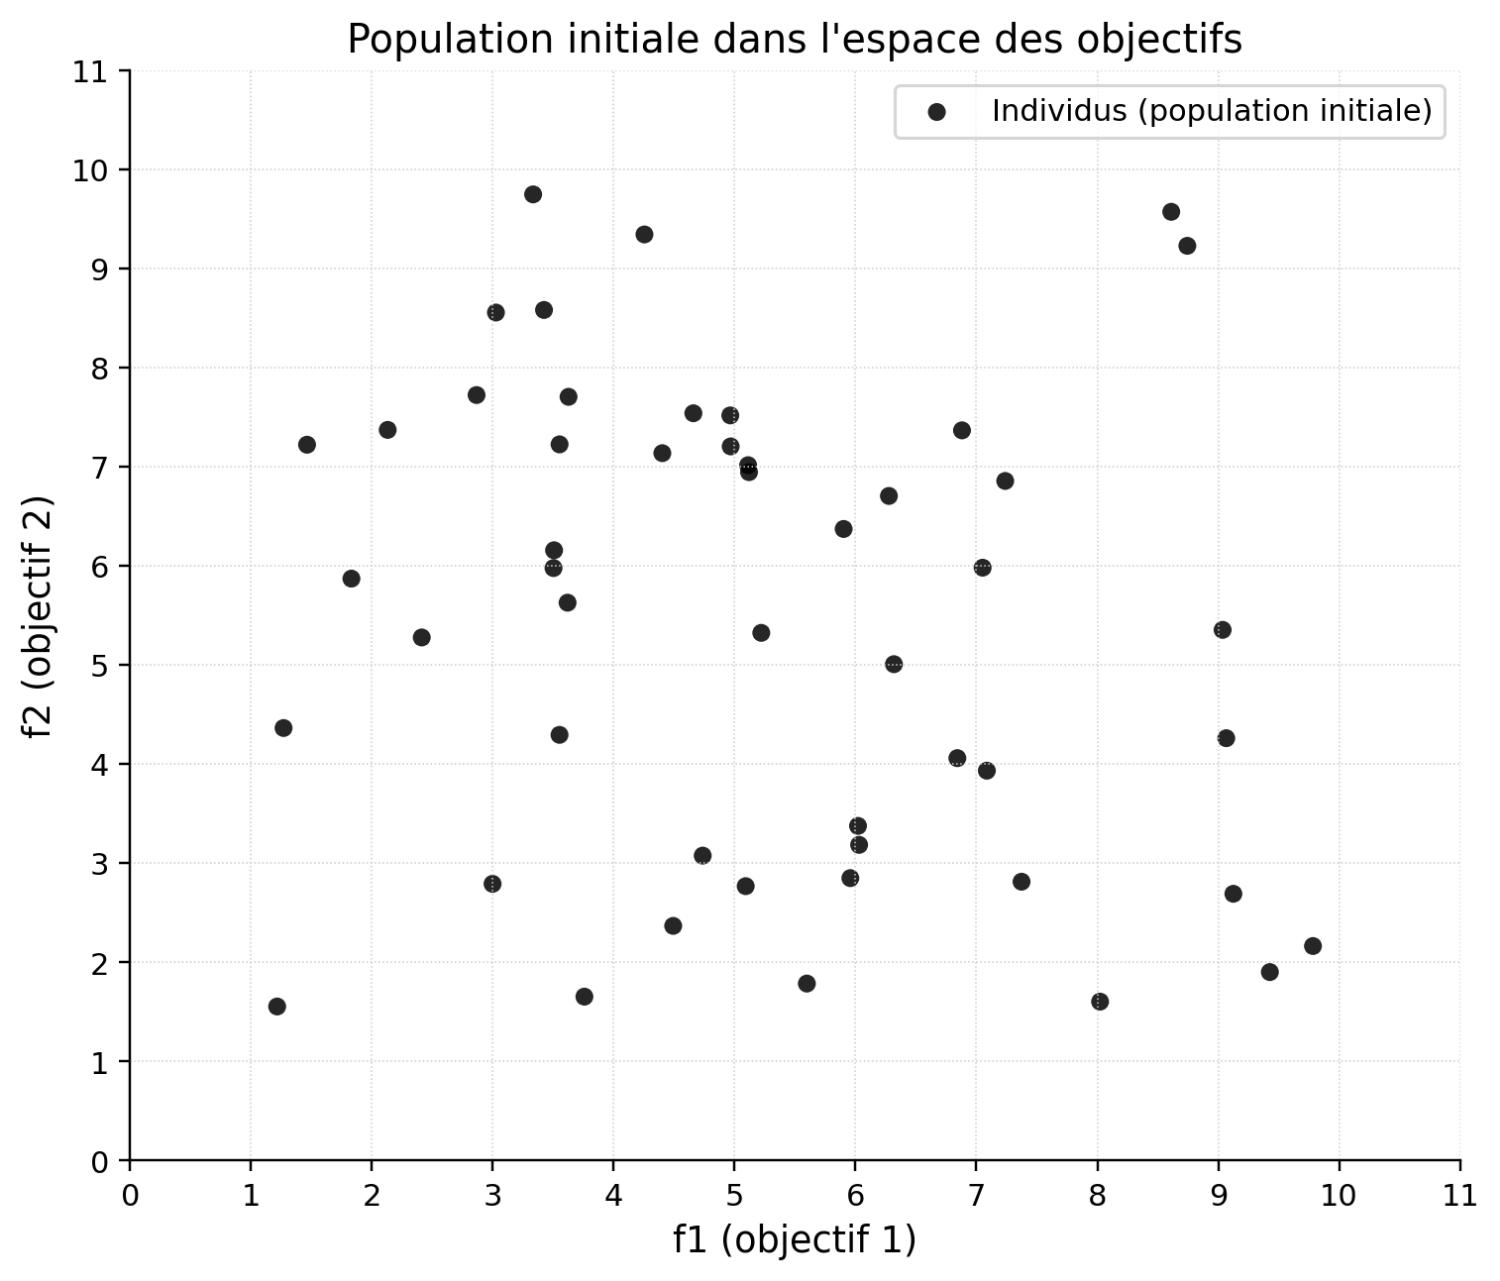
\includegraphics[width=0.65\textwidth]{population_initiale.png}
\caption{Population initiale (espace des objectifs)}
\label{fig:pop_init}
\end{figure}

\textbf{Étape 2 : Tri non-dominé.}

Les individus sont classés en \textbf{fronts successifs} : front 1 (non dominés), front 2 (non dominés après retrait du front 1), etc. Chaque individu reçoit un \textbf{rang} correspondant à son front. Plus le rang est bas, la solution est meilleure.

\begin{figure}[H]
\centering
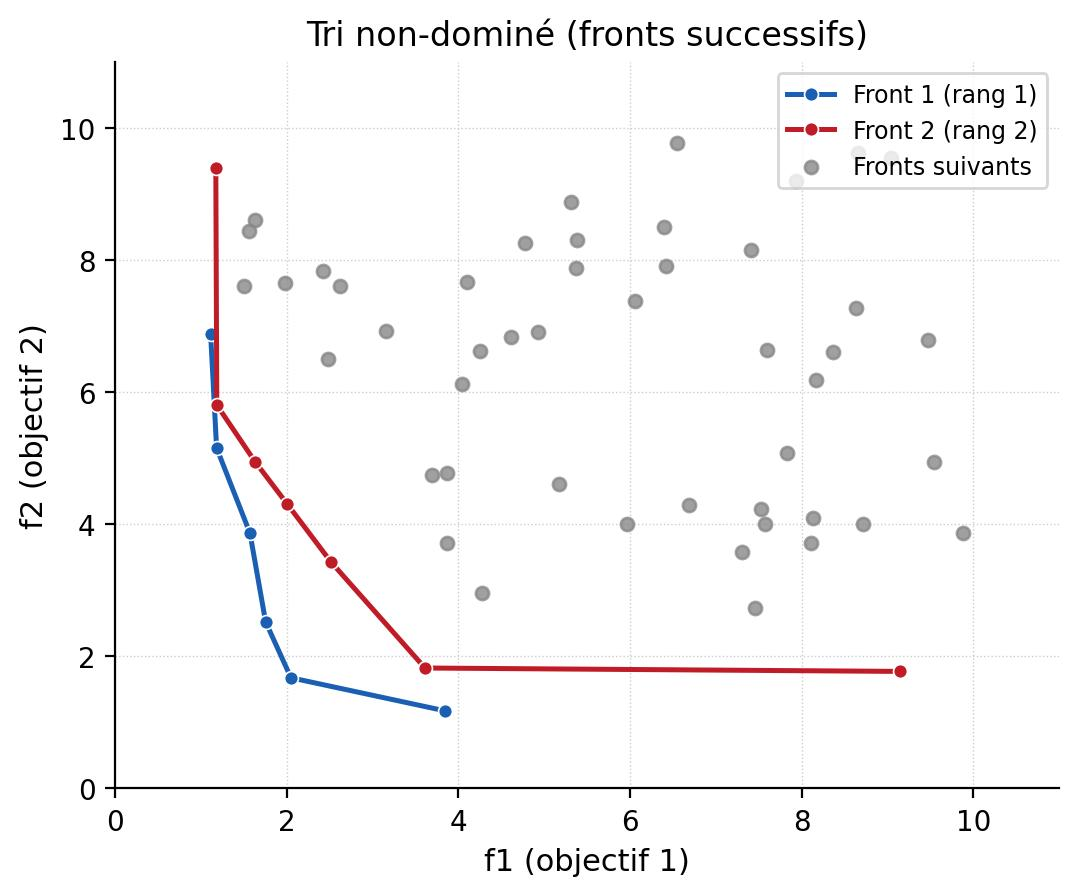
\includegraphics[width=0.70\textwidth]{tri_non_domine.png}
\caption{Tri non-dominé en fronts successifs}
\label{fig:tri}
\end{figure}

\textbf{Étape 3 : Distance de peuplement.}

Pour préserver la \textbf{diversité} du front, NSGA-II calcule pour chaque individu une \textbf{distance de peuplement} : la distance moyenne qui le sépare de ses voisins dans l'espace des objectifs. Un individu isolé est préféré à un individu entassé.

\begin{figure}[H]
\centering
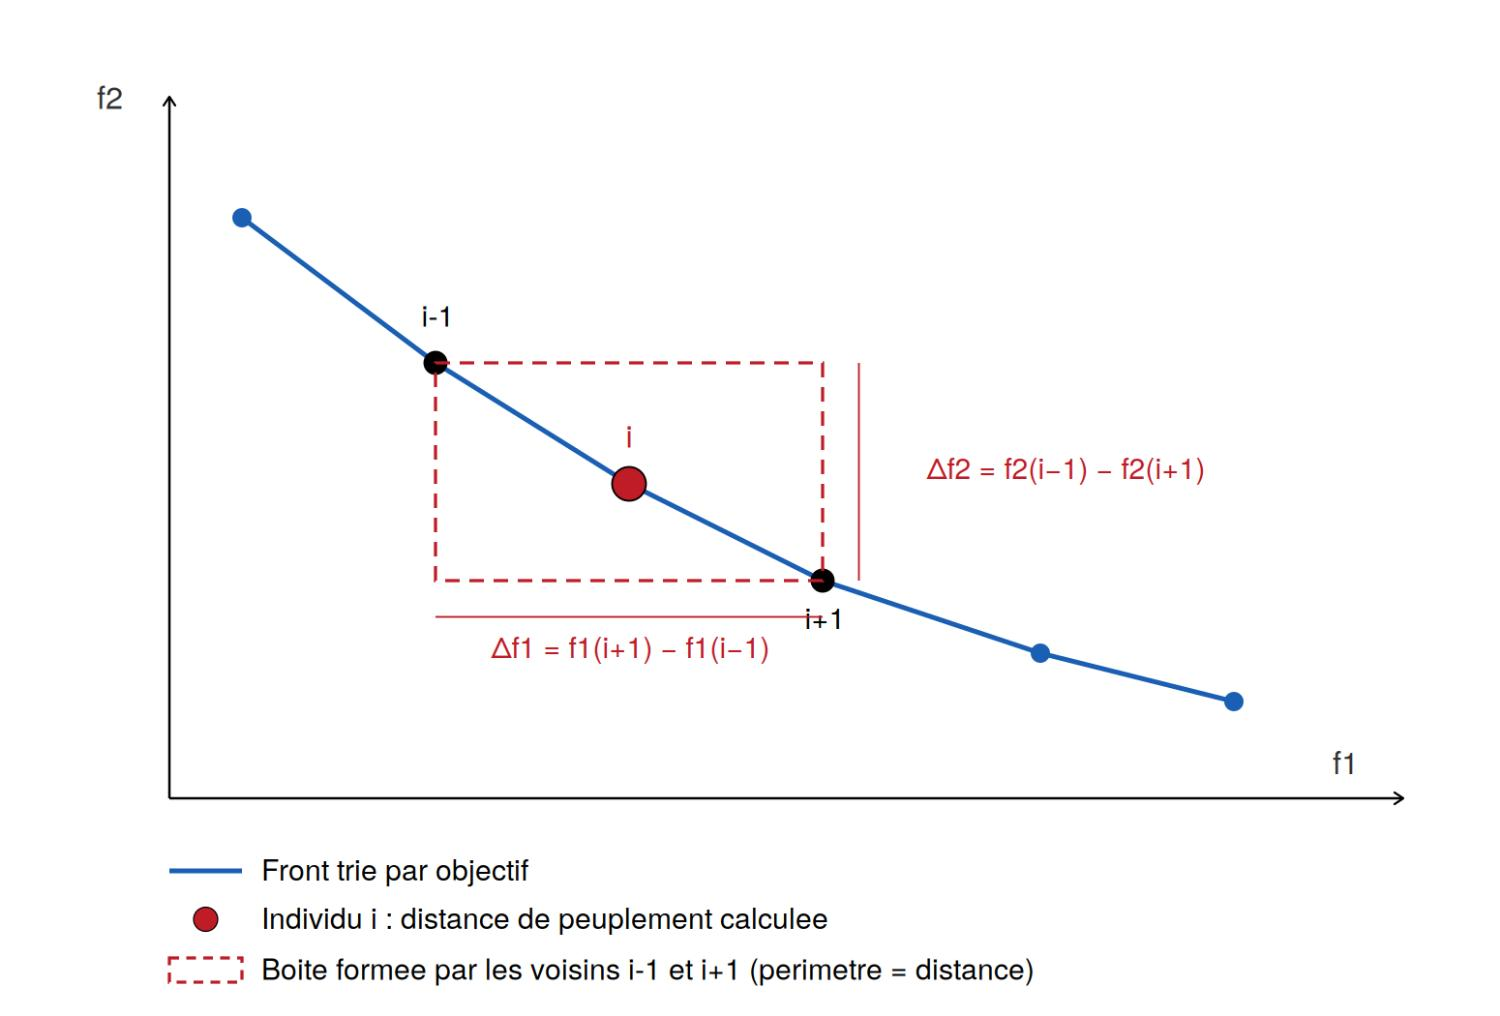
\includegraphics[width=0.72\textwidth]{distance_peuplement.png}
\caption{Distance de peuplement}
\label{fig:distance}
\end{figure}

\textbf{Étape 4 : Sélection des parents.}

Les individus sont sélectionnés par \textbf{tournoi binaire}. Le critère est : d'abord le rang (le plus bas est préféré), puis la distance de peuplement (la plus élevée est préférée). Ce mécanisme favorise à la fois la \textbf{convergence} et la \textbf{diversité}.

\textbf{Étape 5 : Croisement et mutation.}

Les parents sont croisés deux à deux pour produire des enfants. L'opérateur dépend du codage : croisement barycentrique (SBX) pour le réel, croisement d'ordre (OX) ou partiellement apparié (PMX) pour les permutations. Les enfants subissent ensuite une \textbf{mutation} aléatoire (taux typique : 5 à 10 \%).

\textbf{Étape 6 : Combinaison parents et enfants.}

Les deux populations ($N$ parents + $N$ enfants) sont \textbf{fusionnées} pour former une population temporaire de $2N$ individus. Cette étape garantit l'\textbf{élitisme}.

\textbf{Étape 7 : Tri non-dominé de la population combinée.}

La population combinée est triée selon le même principe. La nouvelle population de $N$ individus est remplie en prenant les fronts dans l'ordre. Si un front dépasse la place restante, les individus \textbf{les mieux répartis} sont sélectionnés selon leur distance de peuplement.

\textbf{Étape 8 : Répétition.}

Les étapes 2 à 7 sont répétées sur un nombre fixé de générations ou jusqu'à un critère d'arrêt. La population finale contient le \textbf{front de Pareto} approximé.

\begin{figure}[H]
\centering
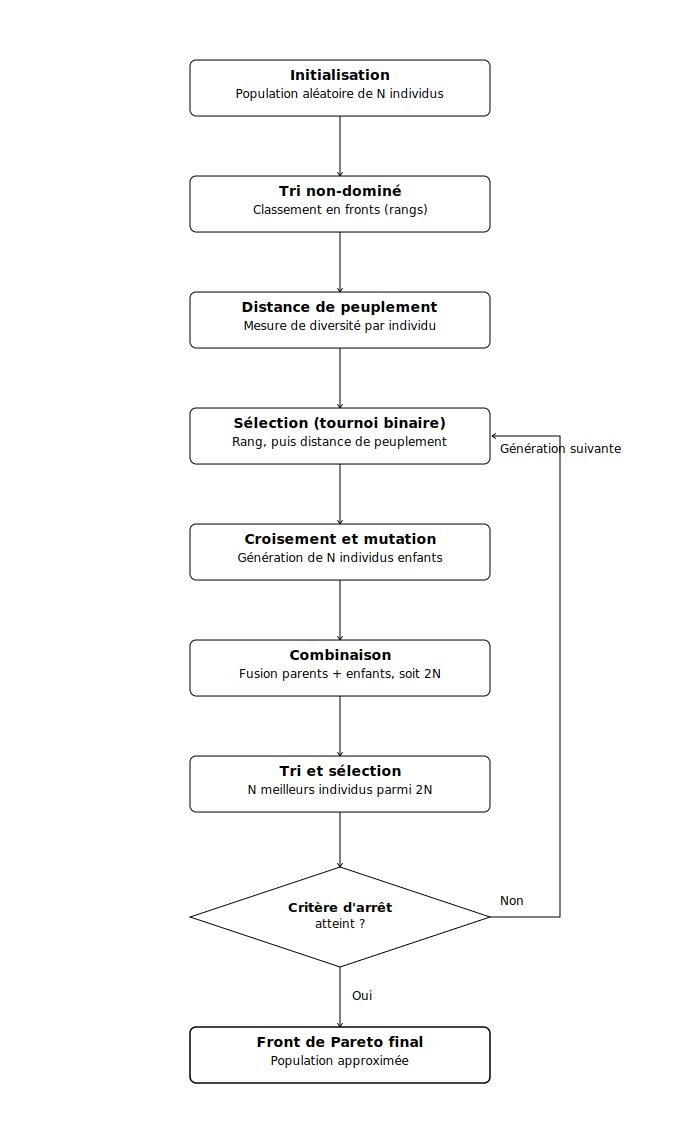
\includegraphics[width=0.58\textwidth]{organigramme_nsga2.png}
\caption{Organigramme de NSGA-II}
\label{fig:nsga2}
\end{figure}



\subsubsection{Avantages et limites}

\begin{itemize}
\item \textbf{Avantages} : convergence rapide, bonne répartition des solutions, élitisme, complexité maîtrisée $O(M N^2)$.
\item \textbf{Limites} : efficacité décroissante au-delà de 3 objectifs, sensibilité au réglage des paramètres, pas de garantie d'optimalité globale.
\end{itemize}

\section{Robustesse d'une trajectoire}

La planification de trajectoire présentée dans les sections précédentes repose sur un \textbf{modèle nominal} du robot et de son environnement. En pratique, le modèle n'est qu'une approximation : les paramètres physiques sont incertains, les mesures sont bruitées, et des perturbations externes peuvent survenir en cours d'exécution. La \textbf{robustesse} désigne la capacité d'une trajectoire à rester performante malgré ces incertitudes.

\subsection{Sources d'incertitude}

Les incertitudes qui affectent la planification et l'exécution d'une trajectoire robotique peuvent être classées en trois familles \cite{puphal2026} :

\begin{itemize}
\item \textbf{Incertitudes de modèle.}
Le modèle géométrique et dynamique du robot est une approximation de la réalité. Les paramètres physiques (masses, inerties, longueurs, raideurs) sont connus avec une précision limitée, et certains phénomènes (frottements, élasticité, jeu mécanique) sont négligés ou simplifiés. Dans le cas des robots à câbles, l'élasticité des câbles et leur affaissement sous poids propre introduisent des écarts entre le modèle rigide et le comportement réel \cite{khayour2022}.

\item \textbf{Incertitudes de mesure.}
Les capteurs (codeurs, accéléromètres, capteurs de force) fournissent des mesures entachées de bruit, avec une résolution et une bande passante finies. L'estimation de la pose réelle de la plateforme à partir de ces mesures est donc imparfaite, ce qui peut conduire à des erreurs de suivi de trajectoire.

\item \textbf{Perturbations externes.}
L'environnement d'exécution peut être source de perturbations non modélisées : vent, vibrations du bâti, chocs, variations de température. Ces perturbations sont critiques pour les robots à câbles, dont la faible rigidité les rend sensibles aux efforts extérieurs \cite{khayour2022}. Une rafale de vent peut faire chuter la tension d'un câble sous son seuil minimal et compromettre la stabilité du système.
\end{itemize}

\begin{figure}[H]
\centering
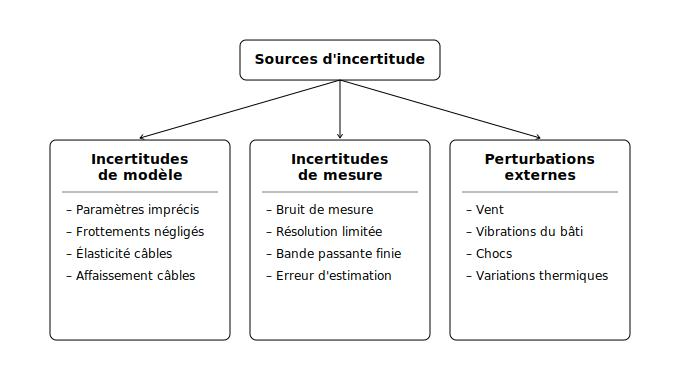
\includegraphics[width=0.85\textwidth]{incertitude.png}
\caption{Sources d'incertitude}
\label{fig:incertitudes}
\end{figure}

\section*{Conclusion}

Ce chapitre a présenté les fondements théoriques de la planification et de l'optimisation de trajectoires, en distinguant path planning et trajectory planning, et en détaillant les méthodes de génération de chemin, de lissage, les contraintes mécaniques, cinématiques, de visibilité et de stabilité, ainsi que le cadre d'optimisation mono- et multi-objectif et les stratégies de robustesse. Les principales approches ont été décrites, comme la couverture complète, la tournée de points, le profil LSPB, le front de Pareto et l'algorithme NSGA-II. Ce cadre général reste indépendant de tout système physique particulier : il ne permet pas encore de choisir entre les différentes méthodes, ni d'anticiper les contraintes propres à un robot à câbles telles que la faible rigidité ou les limites de tension. C'est cette confrontation à un cas concret qui doit permettre de sélectionner, parmi les outils présentés, ceux les mieux adaptés à ces contraintes spécifiques. Le chapitre suivant est ainsi consacré à l'étude du robot Tandem, qui applique ces concepts à un système réel et en tire les choix méthodologiques correspondants.




\clearpage
% ============================================================
% CHAPITRE III
% ============================================================
